\documentclass[a4paper,12pt,oneside]{report}
\usepackage{graphicx}
%font=default,size 12pt
%Configure page layout: a4, margin 1in, noheader, nofooter
\paperwidth=8.26in
\paperheight=11.69in
\pagestyle{empty}
\voffset=-0.5in
\hoffset=-0.5in
\oddsidemargin=0in
\evensidemargin=0in
\topmargin=0in
\headheight=0in
\headsep=0in
\marginparsep=0in
\marginparwidth=0in
\footskip=0in
\marginparpush=0in
\textwidth=7.26in
\textheight=10.69in
%indent of a first line of new paragraphc is 1cm to use \indent or \par
\parindent=1cm
%set distance btw lines
\baselineskip=0pt
%set disctance btw pars
\parskip=0pt
%create a listing environment for arranging text
%tree level 1: {\textbullet}{0in}{0in}{\parindent}
%tree level 2: dependent :D
\newenvironment{tree}[4]{
\begin{list}{#1}{\parskip=0in \topsep=0in \itemsep=0in \parsep=0in \partopsep=0in \leftmargin=#2 \rightmargin=#3 \itemindent=#4 \listparindent=\itemindent}
}{\end{list}}
%creat a small standalone section document :D
\newenvironment{sasection}[3]{
\framebox{\textbf{#1}} \underline{\textbf{#2}}
\begin{tree}{#3}{0in}{0in}{\parindent}
}{\end{tree}}
%creat a small section document beyond some levels:D
\newenvironment{ssection}[5]{
\phantom{#1}\textbf{#2\space#3}
\begin{tree}{#4}{0in}{0in}{#5}
}{\end{tree}}
%fix other errors manually if needed: line break, etc.
\begin{document}
\centerline{\framebox{\textbf{{\Huge Mechanical Oscillations}}}}\ \\ \par \noindent
\framebox{\textbf{1}} \textbf{\underline{Periodic motions and simple harmonic motions}} \\
\begin{ssection}{\quad}{1}{Periodic motions and oscillations}{\textbullet}{\parindent}
\item Periodic motion is motion of an object in which the object returns to a given position after a fixed time interval.
\item An oscillation, or vibration, is a limited motion on a space, repeating back and forth many times around an equilibrium position where thing is at rest.
\item Periodic oscillation is the oscillation whose state is repeated as it was after a constant period of time.\\
\indent The smallest period of time $T$ after that states of oscillation are repeated as they were is called the period of periodic oscillation.\\
\indent The quantity $f=1/T$ showing the number of oscillations (i.e. how many times a state of oscillation is repeated as it were) per unit of time is called the frequency.\\
\indent If time is measured in seconds [s], then frequency is specified in hertz [Hz] = [$s^{-1}$].
\item Of all the oscillatory motions, the most important is simple harmonic motion (SHM), because, besides being the simplest motion to describe mathematically, it constitutes a rather accurate description of many oscillations found in nature.
\end{ssection}\
\begin{ssection}{\space}{2}{Simple harmonic motions}{\textbullet}{\parindent}
\item By definition, a simple harmonic motion (SHM) can be illustrated mathematically. A particle moving along the X-axis has SHM when its displacement $x(t)$ relative to the origin of the coordinate system is given as a function of time by the relation\\ \centerline{$x(t)=X_{m}\cos(\omega t+\phi)$}\\ \indent, where $X_{m}>0$ is the maximum displacement from the origin or the amplitude of the SHM, $\omega>0$ [$rad/s$] is called the angular frequency of the oscillating particle, $(\omega t+\phi)$ is called the phase, and thus $\phi\in R$ is the initial phase. The period $T$ of the SHM as well as its frequency $f$ is related to the angular frequency $\omega$ by $\omega=2\pi f=2\pi/T$.\\
\indent The velocity of the particle $v(t)=\dot{x(t)}=-\omega X_{m}\sin(\omega t+\phi)$.\\
\indent The acceleration is given by $a(t)=\dot{v(t)}=\ddot{x(t)}=-\omega^{2}X_{m}\cos(\omega t+\phi)=-\omega^{2}x(t)$. \\ \indent In general, for a sinusoidally time-varying displacement function $x(t)$, we have,\\ \centerline{$\dot{x}^{2}(t)+\omega^{2}x^{2}(t)=\omega^{2}X^{2}_{m}$ and $\ddot{x}(t)+\omega^{2}x(t)=0$.}
\item The second-order linear differential equation: $\ddot{x}(t)+\omega^{2}x(t)=0$, with $\omega\in R$\\ \indent $<=> x(t)=C_{1}\cos(|\omega|t)+C_{2}\sin(|\omega|t)$, with $C_{1}, C_{2} \in R$\\There is an angle $\phi \in [-\pi,\pi]$ such that $\cos(\phi)=C_{1}/\sqrt{C_{1}+C_{2}}, \sin(-\phi)=C_{2}/\sqrt{C_{1}+C_{2}}$\\So,the given equation $<=> x(t)=\sqrt{C_{1}+C_{2}}\cos(|\omega|t+\phi)$\\ \indent If we assume $x(t)$ as a displacement function of a motion with respect to $t$ taken as time variable, then, based on the definition of SHM, $x(t)$ represents a SHM with its angular frequency of $|\omega|>0$, its amplitude of $X_{m}=\sqrt{C_{1}+C_{2}}>0$, and its initial phase of $\phi\in R$.\\ \indent Therefore, the equation $\ddot{x}(t)+\omega^{2}x(t)=0$ with $x(t)$ is a time-varying displacement function of a motion typifies SHM of a particle taking $x(t)$ as its displacement funtion and sinusoidally oscillating with its angular frequency of $|\omega|$.
\item The SHM of a particle with its displacement function given by either $x(t)=X_{m}\cos(\omega t+\phi)$ or $x(t)=X_{m}\sin(\omega t+\phi)$ can be considered as the orthogonal projection of a point $M$ represented by a vector $\overrightarrow{OM}=\vec{x}$, rotating counterclockwise around $O$ with constant radius $|\vec{x}|=X_{m}$ and constant angular velocity $\omega$, and making at each instant an angle $(\omega t+\phi)$ onto either X-axis or Y-axis respectively in the Cartesian coordinate system.\\
\indent $\vec{x}(t)=X_{m}e^{i(\omega t+\phi)}=X_{m}\angle(\omega t+\phi)=X_{m}(\cos(\omega t+\phi),\sin(\omega t+\phi))$\\ \indent\phantom{ $\vec{x}(t)$}$=X_{m}\vec{u}_{r}$ (in the polar coordinate system)\\
\indent$\rightarrow \vec{v}(t)=\displaystyle\frac{d\vec{x}(t)}{dt}=i\omega X_{m}e^{i(\omega t+\phi)}=\omega X_{m}\angle(\omega t+\phi+\frac{\pi}{2})=\omega X_{m}\left[\begin{array}{c}-\sin(\omega t+\phi)\\\cos(\omega t+\phi)\end{array}\right]^{T}$\\ \indent\phantom{$\rightarrow \vec{v}(t)=\displaystyle\frac{d\vec{x}(t)}{dt}$} $=X_{m}d\vec{u}_{r}/dt=X_{m}(d\Phi/dt)\vec{u}_{\Phi}=\omega X_{m}\vec{u}_{\Phi}$\\
\indent$\rightarrow \vec{a}(t)=\displaystyle\frac{d\vec{v}(t)}{dt}=-\omega^{2}X_{m}e^{i(\omega t+\phi)}=-\omega^{2}X_{m}\angle(\omega t+\phi)=-\omega^{2}X_{m}\left[\begin{array}{c}\cos(\omega t+\phi)\\\sin(\omega t+\phi)\end{array}\right]^{T}$\\ \indent\phantom{$\rightarrow \vec{a}(t)=\displaystyle\frac{d\vec{v}(t)}{dt}$}
$=\omega X_{m}d\vec{u}_{\Phi}/dt=-\omega X_{m}(d\Phi/dt)\vec{u}_{r}=-\omega^{2}X_{m}\vec{u}_{r}$\\
\indent In uniform circular motion, it is clear that $\vec{a}=i\omega\vec{v}=-\omega^{2}\vec{x} \rightarrow \vec{v}\perp\vec{a}\parallel\vec{x}$\\, where $\vec{x}=X_{m}\angle(\omega t+\phi)$ represents the position of the given particle $M$.\\
\begin{tabular}{ccp{0.175\textwidth}}
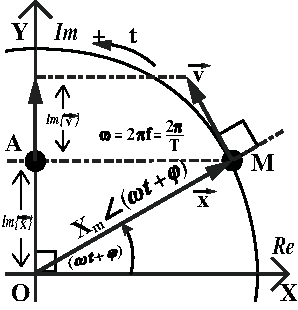
\includegraphics[scale=1.4]{figures/1Dec2.pdf}
&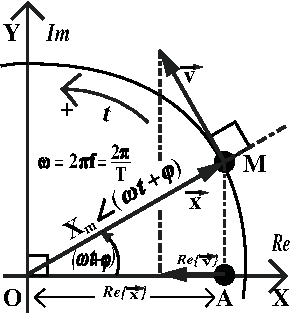
\includegraphics[scale=1.4]{figures/1Dec1.pdf}
&\begin{minipage}[b]{0.175\textwidth}
In general, a simple harmonic oscillation can be considered as the projection of an uniform circular motion onto any straight line in the same plane.\vspace{1in}
\end{minipage}
\end{tabular}
\end{ssection}\
\begin{ssection}{\space}{3}{Force and energy in SHM}{\textbullet}{\parindent}
\item Suppose a particle of mass $m$ oscillating with SHM is located by a displacement function $x(t)$, then $\ddot{x}(t)+\omega^{2}x(t)=0$ must be satisfied. Applying Newton's second law of motion $\vec{F}=m\vec{a}=m\vec{\ddot{x}}$, the force acting on the particle must be $F(t)=-kx(t)$, with $k=m\omega^{2}$ or $\omega=\sqrt{k/m}$. This indicates that in SHM the force is proportional to the displacement, and opposed to it. Thus, the force is always pointing toward the equilibrium position chosed as the origin. The force given by the expression $F(x)=-kx$ with $k=const$ is the type of force in force fields defined in terms of the potiential energy.
\item Given a particle of mass $m$ having the displacement function $x(t)$, moving under effect of the force $F(x(t))=-kx(t)$, with constant $k\in R^{+}$. Applying Newton's second law of motion $\vec{F}=m\vec{a}=m\vec{\ddot{x}}$, we have $a(t)=-kx(t)/m$ or $\ddot{x}(t)+(k/m)x(t)=0$, which means that the particle is oscillating sinusoidally with its angular frequency $\sqrt{k/m}$.
\item The kinetic energy of the particle is $E_{k}(t)=\frac{1}{2}mv^{2}(t)=\frac{1}{2}m\omega^{2}(X_{m}^{2}-x^{2}(t))$\\
\indent Assume the zero of the potential energy at the equilibrium position (the origin) $E_{p}(x=0)=0$, then the potential energy of the particle is\\\centerline{$E_{p}(x(t))=E_{p}(x(t))-E_{p}(0)=\displaystyle-\Delta W_{\overrightarrow{OX}}=-\int_{0}^{x(t)}{F(x(t))dx(t)} <=> E_{p}(x(t))=\frac{1}{2}kx^{2}(t)$}\\
\indent Adding two expressions above, we obtain, for the total energy of SHM:\\\centerline{$E(x(t))=E_{k}(x(t))+E_{p}(x(t))=\frac{1}{2}m\omega^{2}(X_{m}^{2}-x^{2}(t))+\frac{1}{2}kx^{2}(t)=\frac{1}{2}m\omega^{2}X^{2}_{m}=\frac{1}{2}kX_{m}^{2}$}\\
\indent Therefore, it is said that, during a SHM, there is a continuous exchange of kinetic and potential energies. In moving away from the equilibrium position, potential energy increases at the expense of kinetic energy, the reverse happens when the particle moves toward the equilibrium position,but the total energy $E=\frac{1}{2}kX_{m}^{2}$ is conserved over time.
\end{ssection}\
\begin{ssection}{\space}{4}{A spring-mass system}{\textbullet}{\parindent}
\item Given a horizontal spring-mass system with ideal conditions; in equilibrium, the spring exerts no force on the object. Let the equilibrium position be the origin ,and the positive direction be from left to right. When the object is displaced an amount $x$ from its equilibrium position, the spring exerts a\\
\begin{tabular}{p{0.6\textwidth}p{0.4\textwidth}}
force, as given by Hooke's law: $F(x)=-kx$, where $k$ is the elastic constant of the spring, a measure of the spring's stiffness, and $x$ stands for the position of the object to the equilibrium point chosen as the origin. Let $m$ is the mass of the&\raisebox{-48pt}[0in][0in]{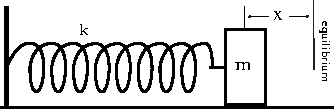
\includegraphics[scale=1,width=0.375\textwidth]{figures/13Dec1.pdf}}
\end{tabular}\\
object. The force on the object indicates the motion in the system is SHM. Therefore, the given spring-mass system has all characteristics of SHM with angular frequency $\sqrt{k/m}$.
\item Given a downward vertical spring-mass system (the reverse of this system can be dealt similarly) in ideal conditions, if the downward direction is chosen to be positive and the no-mass equilibrium (when the spring is unstretched) is taken as the origin, the spring's force on the object is $F_{s}=-ky$, where $y$ is the coordinate of the end of the spring to the origin. Then Newton's second law gives $m\ddot{y}(t)=-ky(t)+mg$.Set a new variable $x=y-\Delta x_{0}$, where $\Delta x_{0}=mg/k$ is the amount the spring is\\
\begin{tabular}{p{0.85\textwidth}p{0.15\textwidth}}
stretched when the object is in its equilibrium (the system equilibrium) chosen as the new origin, so that every position having coordinate $y$ is now represented by new corresponding coordinate $x$ with the new origin. Thus, $md^{2}(x(t)+\Delta x_{0})/dt^{2}=-k(x(t)+\Delta x_{0})+mg=-kx(t)$ or $\ddot{x}(t)+(k/m)x(t)=0$, which states the system's phenomenon is SHM with angular frequency $\sqrt{k/m}$. Moreover, the effect of the gravitational force $mg$ is merely to shift the equilibrium position from $y=0$ to $x=0$, and the unbalanced force is now $-kx$. Therefore, the phenomenon of the given system is SHM about the system equilibrium position ($mg/k$ away from the unstretched equilibrium position of the spring) with the angular frequency $\sqrt{k/m}$, the same as that for an object on a horizontal spring-mass system with elastic constant $k$ in ideal conditions.&\raisebox{-140pt}[0in][0in]{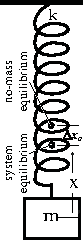
\includegraphics[width=0.11\textwidth,height=150pt]{figures/13Dec2.pdf}}
\end{tabular}
\end{ssection}\
\begin{ssection}{\space}{5}{A pendulum}{\textbullet}{\parindent}
\item A simple pendulum consists of a string of length $l$ and a bob of mass $m$. When the bob is released from an initial angle $\phi_{0}$ with the vertical, it swings back and forth with some period T. The forces on the bob are its weight $m\vec{g}$ and the string tension $\vec{T}$. At an angle $\phi(t)$ with the vertical, the weight has components $mg\cos\phi(t)$ along the string and $mg\sin\phi(t)$ tangential to the circular arc in the direction of\\
\begin{tabular}{p{0.12\textwidth}p{0.85\textwidth}}
\raisebox{-128pt}[0in][0in]{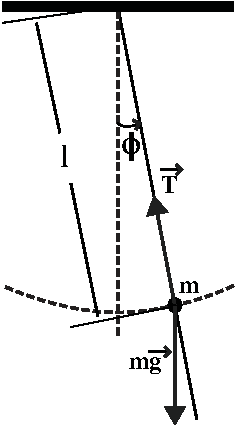
\includegraphics[width=0.13\textwidth,height=136pt]{figures/13Dec3.pdf}}
& decreasing $|\phi(t)|$. Let $s(t)$ be the coordinate of the bob along its orbit with regard to the bottom of the orbit chosen as the origin, and the positive direction is from left to right. Thus, $\phi(t)$ is the angle from the vertical to the direction of the string with the positive direction is counterclockwise, then $s(t)=l\phi(t)$, where $\phi(t)$ is in radians. The tangential component of Newton's second law gives $md^{2}s(t)/dt^{2}=-mg\sin\phi(t)<=>d^{2}\phi(t)/dt^{2}=-g\sin\phi(t)/l$. For small $\phi$, $\sin\phi\approx\phi$, then $\ddot{\phi}(t)+(g/l)\phi(t)=0$. Therefore, as long as the maximum amplitude is small, the given pendulumn oscillates with SHM having angular frequency $\sqrt{g/l}$; also the period, and the frequency, are independent of the amplitude of oscillation, a general feature of SHM.
\end{tabular}
\item Consider a simple pendulum suspended from the ceiling of a boxcar that has acceleration $\vec{a}_{0}$ to the right. Relative to the boxcar, the bob appears to be acted on by a horizontal pseudoforce $-m\vec{a}_{0}$ to the left, in addition to the downward force of gravity $mg$. Using Newton's laws, the equilibrium\\
\begin{tabular}{p{0.84\textwidth}p{0.12\textwidth}}
angle (from the vertical to the string with conventionally counterclockwise as positive direction) is given by $\tan\phi_{0}=-a_{0}/g$. So, relative to the boxcar, all objects will fall at an angle $\phi_{0}$ to the vertical with acceleration $\vec{g}'=\vec{g}-\vec{a}_{0}$. Therefore, Newton's laws can be used relative to the accelerating boxcar by replacing the acceleration due to gravity $\vec{g}$ by $\vec{g}'=\vec{g}-\vec{a}_{0}$. If the bob is displaced slightly from the equilibrium $\phi(t)\neq\phi_{0}$, it will oscillate sinusoidally with its angular frequency $\sqrt{g'/l}$.
&\raisebox{-84pt}[0in][0in]{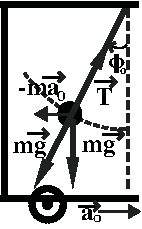
\includegraphics[scale=0.85]{figures/14Dec1.pdf}}
\end{tabular}\\
\indent In general, given a simple pendulum disturbed from its equilibrium angle in an accelerated reference frame, then, as long as the maximum amplitude is small, relative to the frame, the pendulum will oscillate with SHM having angular frequency $\sqrt{g'/l}$, with $\vec{g'}=\vec{g}-\vec{a}_{0}$, where $\vec{a}_{0}$ is the acceleration of the frame with regards to its corresponding non-accelerated ertial frame.
\item A rigid object pivoted about a point other than its center of mass will oscillate\\
\begin{tabular}{p{0.82\textwidth}p{0.2\textwidth}}
when displaced from equilibrium. Such a system is called a physical pendulum.\newline
Consider an object pivoted about a point a distance d from its center of mass and displaced from equilibrium by the angle $\phi_{0}$. The torgue about the pivot $\tau(t)=|\vec{d}(t)\times M\vec{g}|= -Mgd\sin\phi(t)$ ($\vec{d}(t)$ is from the pivot to the object's centre of mass) tends to decrease $|\phi(t)|$. Newton's law applied to rotation is $\tau(t)=I\alpha(t)$, where $\alpha(t)=d^{2}\phi(t)/dt^{2}$ is the angular acceleration, and $I$ is the moment of inertia about the pivot point. Then, $-Mgd\sin\phi(t)=Id^{2}\phi(t)/dt^{2}<=>d^{2}\phi(t)/dt^{2}+(Mgd/I)\sin\phi(t)=0$
&\raisebox{-96pt}[0in][0in]{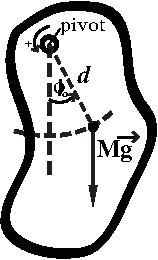
\includegraphics[scale=1.1]{figures/14Dec2.pdf}}
\end{tabular}\\
Again, if the angular displacements are small, so the approximation $\sin\phi(t)\approx\phi(t)$ holds, and $d^{2}\phi(t)/dt^{2}+(Mgd/I)\phi(t)=0$ thus indicates that the motion is SHM with angular frequency $\sqrt{Mgd/I}$.
\end{ssection}\ \par\noindent
\framebox{\textbf{2}} \textbf{\underline{Damped oscillations, driven oscillations and resonance}} \\
\begin{ssection}{\quad}{1}{Damped oscillations}{\textbullet}{\parindent}
\item In experimental conditions, left to itself, a spring or a pendulum eventually stops oscillating because the mechanical energy is dissipated by frictional forces. Such motion is said to be damped. Damped oscillations whose both the amplitude and the energy, which is proportional to the square\\\indent of the amplitude, decrease by a constant percentage in a given time interval (exponential decrease)\\\phantom{Damped oscillations whose both the }will be discussed here.The force exerted by a damper such\\
\begin{tabular}{lp{0.33\textwidth}l}
\raisebox{-107pt}[0in][0in]{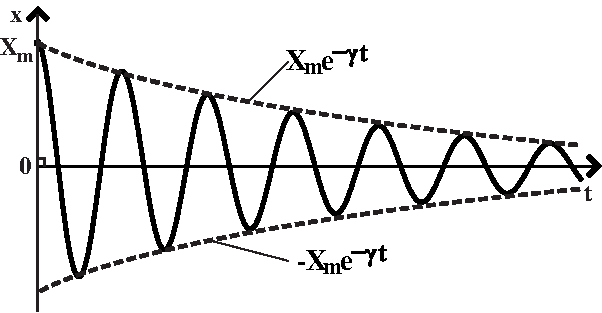
\includegraphics[scale=1]{figures/15Dec1.pdf}}
& as the one shown in the figure can be represented by the empirical expression $\vec{F}_{d}=-\lambda\vec{v}$, where $\lambda$ is a damped constant. Note that other types of damping forces-having other, different, physical relationships may also be present in actual physical situations.
&\raisebox{-107pt}[0in][0in]{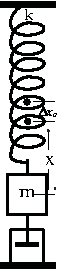
\includegraphics[scale=1]{figures/16Dec1.pdf}}
\end{tabular}\\
\item Applying Newton's laws for an object of mass $m$ on a spring of force constant $k$ under effect of the damper, the differential equation for this damped oscillation is $-kx(t)-\lambda\dot{x}(t)=m\ddot{x}(t)$ or $\ddot{x}(t)+2\gamma\dot{x}(t)+\omega_{0}^{2}x(t)=0$, where $2\gamma=\lambda/m$ and $\omega_{0}=\sqrt{k/m}$ is the natural angular frequency without damping. This type of damped oscillation is often described by its $Q$ factor (for quality factor), $Q=\omega_{0}/(2\gamma)=m\omega_{0}/\lambda$ or $Q=\sqrt{km}/\lambda$. In the case of small damping when $\gamma<\omega_{0}<=>Q>0.5$, the solution then is $x(t)=X_{m}e^{-\gamma t}\cos(\omega t+\phi)$, where $X_{m}$ and $\phi$ are arbitrary constants determined by the initial conditions, and $\omega=\sqrt{\omega_{0}^{2}-\gamma^{2}}=\sqrt{k/m-\lambda^{2}/4m^{2}}=\omega_{0}\sqrt{1-1/(4Q^{2})}$. If the damping is very large, $\gamma$ may become larger than $\omega_{0}$ ($Q\leq0.5$), and $\omega$ becomes imaginary. In this case, there are no oscillations and the particle, if displaced and released, gradually approaches the equilibrium position without crossing it, or, at most crossing it once. 
\end{ssection}\
\begin{ssection}{\space}{2}{Forced oscillations}{\textbullet}{\parindent}
\item Consider an external driving force $f(t)=f_{m}\cos(\omega_{f}t)$ , which is sinusoidally time-varying with its angular frequency $\omega_{f}$, applies on an oscillating object of mass $m$, in addition to the restoring force $-kx(t)$ and a damping force $-\lambda\dot{x}(t)$, then, applying Newton's laws, the object's equation of motion is $ma=-kx-\lambda v+f(t)<=>m\ddot{x}(t)+\lambda\dot{x}(t)+kx(t)=f_{m}\cos(\omega_{f}t)$, which ,if set $2\gamma=\lambda/m$ and $\omega_{0}=\sqrt{k/m}$, can be written in the form $\ddot{x}(t)+2\gamma\dot{x}(t)+\omega_{0}^{2}x(t)=(f_{m}/m)\cos(\omega_{f}t)$. The general solution of this equation consists of two parts: the transient solution that is similar to the solution for the previously mentioned damped oscillation, and the steady-state solution. Over time, the transient solution becomes negligible because of the exponential decrease of the amplitude, so the steady-state solution is taken as the solution here, which is $x(t)=\hat{X}\cos(\omega_{f}t-\phi)$, where $\hat{X}=(f_{m}/m)/\sqrt{(\omega_{0}^{2}-\omega_{f}^{2})^{2}+4\gamma^{2}\omega_{f}^{2}}=f_{m}/\left((k-m\omega_{f}^{2})\sqrt{1+\tan^{2}\phi}\right)$, and $\tan\phi=2\gamma\omega_{f}/(\omega_{0}^{2}-\omega_{f}^{2})$. Note that both the amplitude $\hat{X}$ and the initial phase $\phi$ are no longer arbitratry quantities, but fixed quantities depending on the system's characteristics. If the frequency $\omega_{f}$ of applied force is variable, then the amplitude $\hat{X}$ reaches its maximum $f_{m}/(\lambda\sqrt{\omega_{0}^{2}-\gamma^{2}})$ when $\omega_{f}=\sqrt{\omega_{0}^{2}-2\gamma^{2}}$.
\item When the frequency $\omega_{f}$ of the applied force is equal to $\omega_{0}$, it is said that there is amplitude resonance. The smaller the damping, the more pronounced the resonance, and when $\lambda$ is zero, the resonance amplitude is infinite and occurs at $\omega_{f}=\omega_{0}=\sqrt{k/m}$. At this frequency of the applied force, the velocity, which is now in phase with the applied force, and also the kinetic energy of the oscillation are maximum. In other words, it is said that there is enerygy resonance at which the energy transfer from the applied force to the forced oscillation is at a maximum. 
\end{ssection}
\end{document}